
\chapter{Isoparametric elements}
\section{Partition of the domain}
	\minifig{ch6/1}{ch6/2}{0.4}{0.3}{0.45}{0.45}
	As we have seen, any domain $V$ must undergo a sub-domain $V^e$. In dimension 1 the elements are separated by a point, 2 a curve and 3 a surface. The connection of all elements should be as closely as possible similar to the real domain. Discretization errors can occur for complex geometries. We can solve the issue by decreasing the size of the elements (mesh refreshment) or using elements with curved boundaries (\autoref{ch6/2}). \\
	
	Nodes and elements must satisfiy:
	
	\begin{enumerate}
	\item each element is defined by the coordinates of the nodes located in the element. In the majority of elements available in the litterature, the nodes are on the boundary of the elements. 

	\item  A portion of the boundary between two elements must be identically defined for both elements. 
	\end{enumerate}
	
\section{Classical elements}
	The order of the element is directly related to the number of nodes on its boundary and vice-versa. Most elements are first, second or third-order, enabling to model linear quadradic or cubic boundaries. 
	
	\begin{center}
	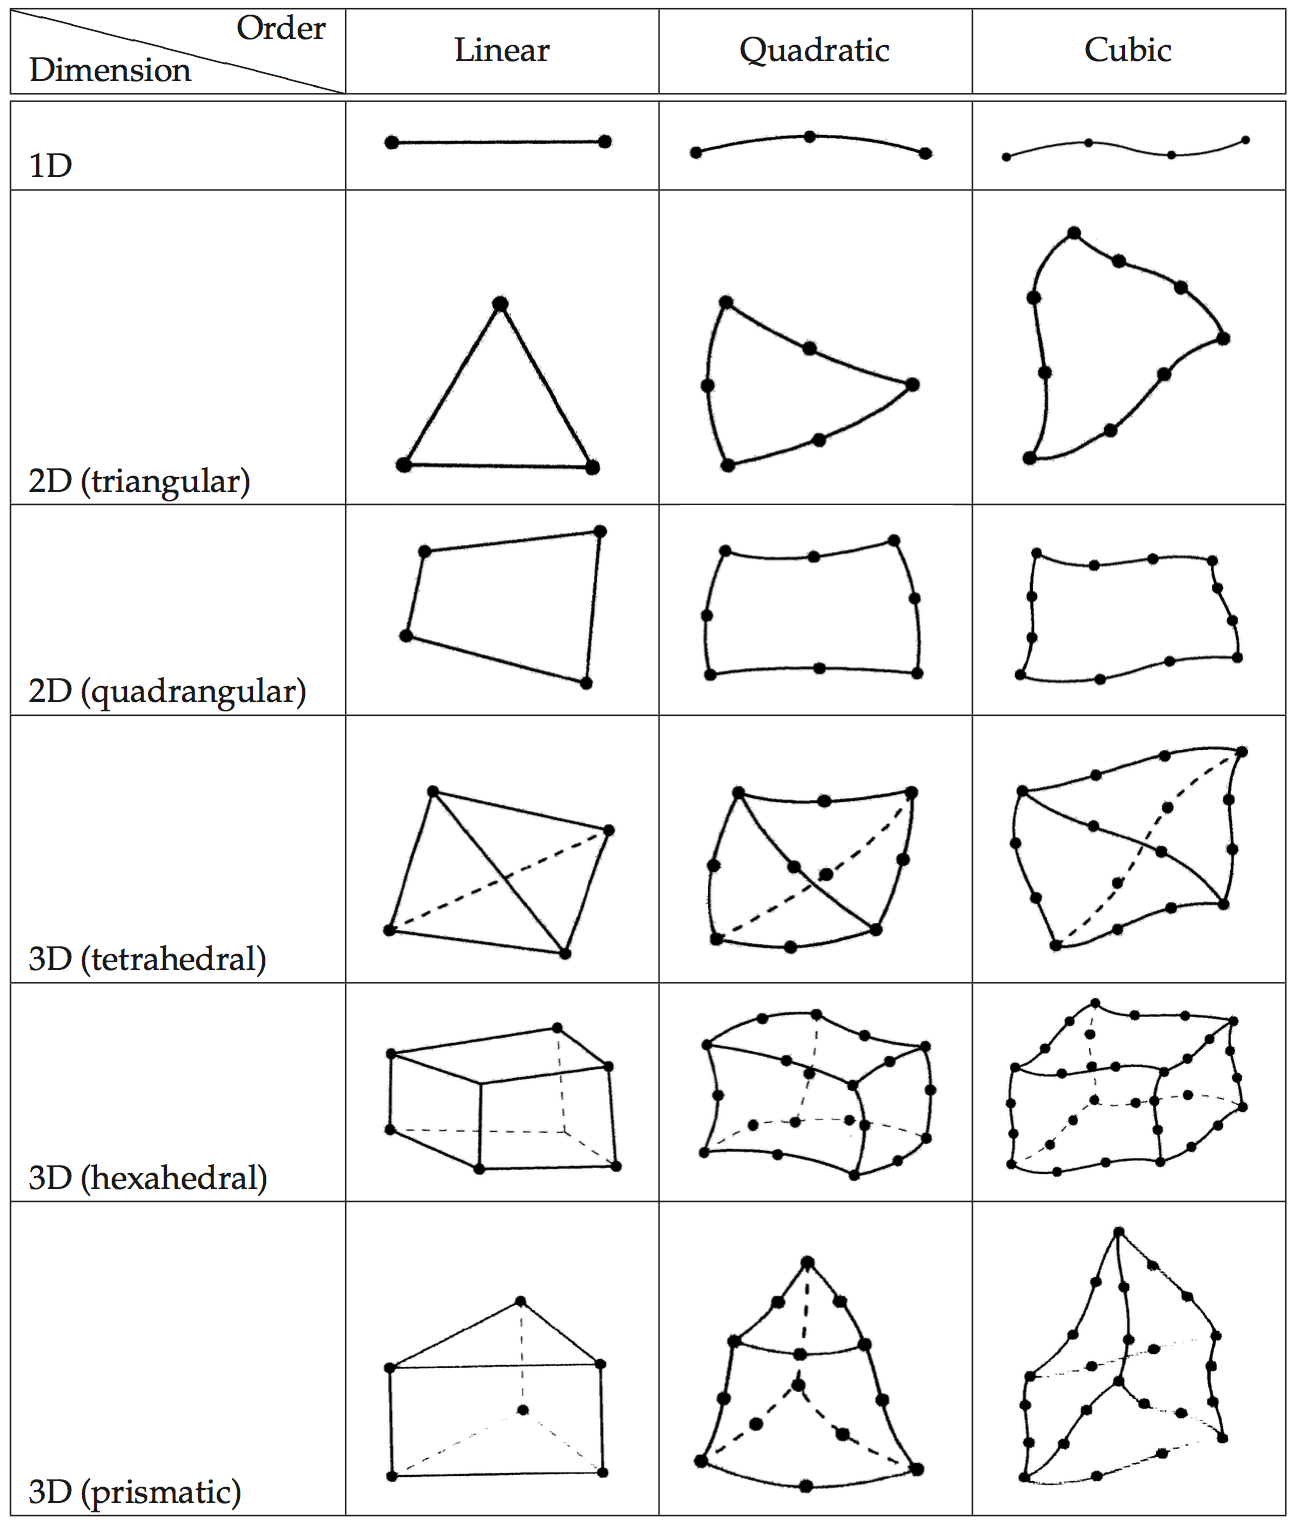
\includegraphics[scale=0.3]{ch6/3}
	\captionof{figure}{}
	\end{center}
	
\section{Reference element and real elements}
	\wrapfig{9}{l}{6}{0.3}{ch6/4}	
	The finite element is the basic element on which the governing equations will be transposed. To avoid complex analytical operations, we will use a \textbf{reference element} on which a mapping of the \textbf{real element} (parent element) has to be performed. By this approach, the shape functions are written for the reference and then converted by linear transformation to the real. In 2D, the reference element is defined over a $(\xi, \eta)$-space, while the real elements are defined over the usual $(x,y)$-space. \\
	
	To perform this operation, a transformation $\mathcal{T}$ is required: 
	
	\begin{equation}
	\mathcal{T} : \xi \rightarrow x{\xi} = \bar{N}^e (\xi) x^e
	\end{equation}
	
	where $x^e$ are the coordinates of the nodes of the element $V^e$ and $\bar{N}^e(\xi)$ are the \textbf{geometric transformation functions} which must follow the same rules as shape functions. This transformation allows to write the analytical definition for each $V^e$ with respect to $\xi$ on a simple element $V^r$. The function $u(x)$ to be approximated can be written as $u(\xi)$. \\
	
	\wrapfig{7}{l}{6}{0.3}{ch6/5}
	Let's make an example with a triangular element. On the figure is represented the reference and the parent element of a three-node triangular element. The reference is defined as:
	
	\begin{equation}
	\xi \geq 0, \quad \eta \geq 0, \quad \xi + \eta \leq 1.
	\end{equation}
	
	\newpage
	Let us consider a real element defined by three nodes $i, j, k$ and the transformation $\mathcal{T}$ such that: 
	
	\begin{equation}
	x(\xi, \eta) = [1-\xi - \eta \quad \xi \quad \eta] 
	\left[
	\begin{array}{c}
	x_i\\
	x_j\\
	x_k
	\end{array}
	\right], 
	\qquad 
	y(\xi, \eta) = [1-\xi - \eta \quad \xi \quad \eta] 
	\left[
	\begin{array}{c}
	y_i\\
	y_j\\
	y_k
	\end{array}
	\right].
	\end{equation}
	
	$\mathcal{T}$ verifies the following properties:
	
	\begin{enumerate}
	\item the nodes (0,0), (0,1) and (1, 0) from $V^r$ are converted into $(x_i, y_i), (x_j, y_j)$ and $(x_k, y_k)$: 
	
	\item each boundary of $V^r$ is transformed into a boundary of $V^e$. For example, the line between (1, 0) and (0, 1) is transformed into $1 -\xi-\eta =0$ or $\eta = 1- \xi$: 
	
	\begin{equation}
	x = [0 \quad \xi \quad 1- \xi] 
	\left[
	\begin{array}{c}
	x_i\\
	x_j\\
	x_k
	\end{array}
	\right] , 
	\qquad 
	y = [0 \quad \xi \quad 1-\xi] 
	\left[
	\begin{array}{c}
	y_i\\
	y_j\\
	y_k
	\end{array}
	\right].
	\end{equation}
	
	\item The transformation is \textbf{bijective}. This is valid only if the Jacobian matrix $\bm{J}$ is not singular:
	
	\begin{equation}
	\bm{J} = \left[
	\begin{array}{cc}
	\frac{\D x}{\D \xi} & \frac{\D y}{\D \xi}\\
	\frac{\D x}{\D \eta} & \frac{\D y}{\D \eta}
	\end{array}
	\right]
	= \left[
	\begin{array}{cc}
	x_j - x_i & y_j - y_i\\
	x_k - x_i & y_k - y_i
	\end{array}
	\right].
	\end{equation}
	
	This is equal to 0 only if the vertices are aligned. 
	\end{enumerate}
	
	\wrapfig{5}{l}{6}{0.3}{ch6/6}
	Geometrically, we can see the $\xi$-variables as a local coordinate system. The process of generating meshes on surfaces is called \textbf{tesselation}. Reference elements are listed on \autoref{ch6/7} and remark that for the 3D case, we have a system $(\xi, \eta, \zeta)$.
	
	\ \\
	\begin{center}
	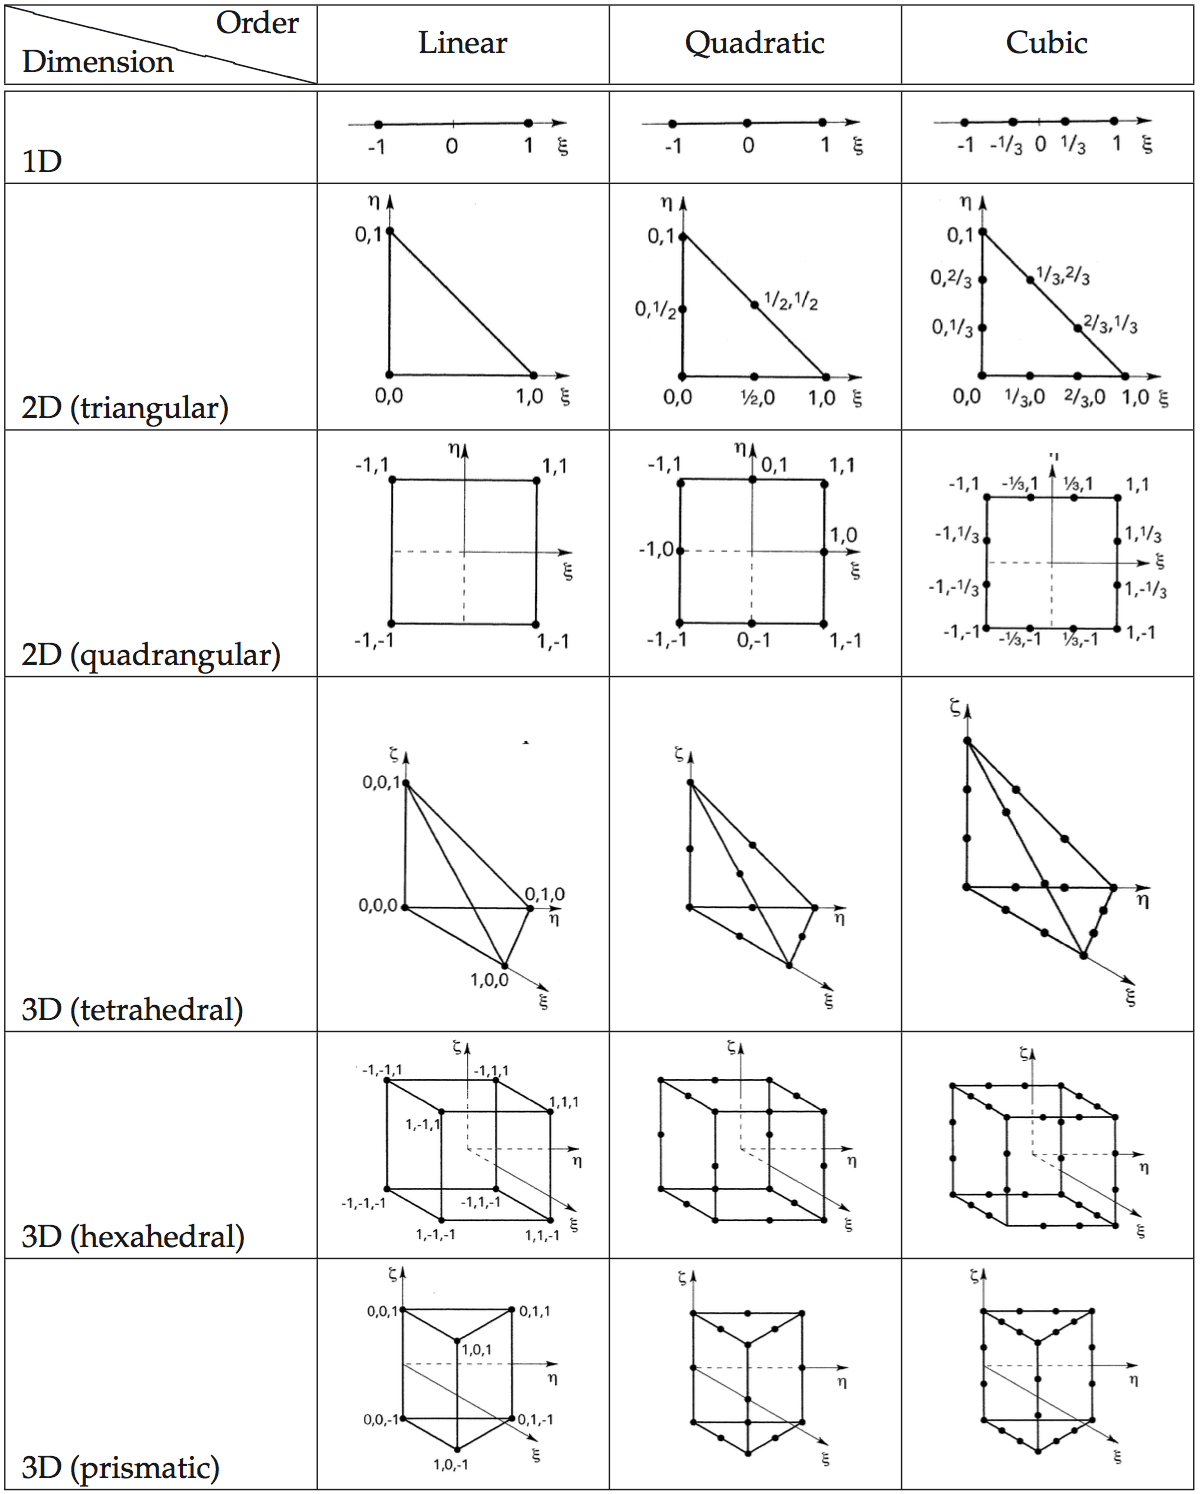
\includegraphics[scale=0.3]{ch6/7}
	\captionof{figure}{}
	\label{ch6/7}
	\end{center}
	
\section{Approximation on the reference element}
	Remind that we want to approximate a quantity of interest $u(\bm{x})$: 
	
	\begin{equation}
	u(\bm{x}) = [N_1(\bm{x}) \quad N_2(\bm{x}) \dots] \left[
	\begin{array}{c}
	u_1\\
	u_2\\
	\vdots
	\end{array}
	\right] = \bm{N^e(x)q^e}
	\end{equation}
	
	This expression is in the real space, using the $\mathcal{T}$ transformation:
	
	\begin{equation}
	u(\bm{\xi}) = \bm{N^e(\xi) q^e}, \qquad \mathcal{T}: \bm{\xi} \rightarrow \bm{x(\xi)} = \bm{\bar{N}^ex^e}.
	\end{equation}
	
	We have 4 properties:
	
	\begin{enumerate}
	\item the approx is \textbf{interpolant}: $u(\xi _i) = u_i$, related to $N_j (\xi _i) = \delta _{ij}$;
	
	\item \textbf{continuity in the element:} the $N_j$ and their derivatives up to the order $s$ must be continuous;
	
	\item \textbf{continuity between elements}: the approx of $u$ and its derivatives up to the order $s$ must depend univocally on the nodal variables appearing on the boundary between the elements and nothing else;
	
	\item when the size of the element tends to 0, the error on the approx and its derivatives vanish. 
	\end{enumerate}
	
	It is also possible to demonstrate that $\sum_i N_i(\bm{\xi}) = 1$. Approx of $C^0$- or $C^s$-type if u or u and its derivatives up to the order $s$ are continuous. Finally, if $\bm{\bar{N} = N}$ the elements are \textbf{isoparametric}. If not:
	
	\begin{itemize}
	\item[•] \textbf{sub-parametric} if the order of polynomials of the geometric transformation is lower than for the shape functions;
	
	\item[•] \textbf{super-parametric} if the order is higher. 
	\end{itemize}
	\ \\
	
	\wrapfig{8}{l}{6.5}{0.3}{ch6/8}
	There can also be \textbf{infinite elements}. They can be devised in 1D by the following mapping: 
	
	\begin{equation}
	x = x_1 + \alpha \frac{1+\xi}{1-\xi}
	\end{equation}
	
	varying from $x=x_1$ to $\infty$ for $\xi$ from -1 to 1. Used for infinite domains like the soil. 
	
\section{Construction of the shape function}
	\wrapfig{6}{r}{6}{0.3}{ch6/9}
	This will be shown for the example of a four-node quadrangular element. We are searching for $\bm{N}^e$ such that $u^e(\bm{x}) = \bm{N^e(x)q^e}$. First a polynomial basis must be set up with $u(\bm{\xi}) = \bm{p(\xi)}^T a$, then by $u(\bm{\xi}) = \bm{p(\xi)}^T a = \bm{N^e}q^e$ we can retrieve the shape functions. A suitable polynomial is the one containing four terms and symmetric wrt $\xi$ and $\eta$: 
	
	\begin{equation}
	\bm{p(x)} = [1\quad \xi \quad \eta \quad \xi \eta].
	\end{equation}
	
	Then the interpolation: 
	
	\begin{equation}
	\bm{q^e} = \left[
	\begin{array}{c}
	u_1\\
	u_2\\
	u_3\\
	u_4
	\end{array}
	\right]
	\left[
	\begin{array}{cccc}
	p_1(\xi _1) & p_2(\xi _1) & p_3(\xi _1) & p_4(\xi _1)\\
	p_1(\xi _2) & p_2(\xi _2) & p_3(\xi _2) & p_4(\xi _2)\\
	\vdots & & & \vdots
	\end{array}
	\right]
	\left[
	\begin{array}{c}
	a_1\\
	a_2\\
	a_3\\
	a_4
	\end{array}
	\right]
	\end{equation}
	
	By inverting the matrix $\bm{P}$, we get the coefficients: $\bm{a = P^{-1}q^e}$. Finally, the shape functions can be obtained as follows: 
	
	\begin{equation}
	u(\bm{\xi}) = \bm{N^e(\xi)q^e = p(\xi)^Ta = p(\xi)^TP^{-1}q^e} \qquad \Rightarrow \bm{N^e(\xi) = p(\xi)^TP^{-1}}.
	\end{equation}